%!TEX root = <cours.tex>
\chapter{Représentation du texte}
\introduction{Peux-tu décoder ce texte ?}

\section{Le code ASCII}


Pour représenter les caractères que nous utilisons pour écrire, on a historiquement choisi d'associer \textit{un numéro} (ou code) à chacun de
ces caractères. La correspondance entre chaque caractère et son code était appelée un \textit{Charset}.\\
Puisqu'à l'origine seul un petit nombre de caractères était utilisé (les caractères de base anglo-saxons), un octet suffisait pour les
représenter tous.\\
Le fait de représenter en machine un jeu de caractères s'appelle réaliser un encodage (\textit{encoding} en Anglais).\\

Le premier encodage utilisé fut l'\textsc{ASCII}, qui signifie  \textit{American Standard Code for Information Interchange}.\\

\begin{center}
    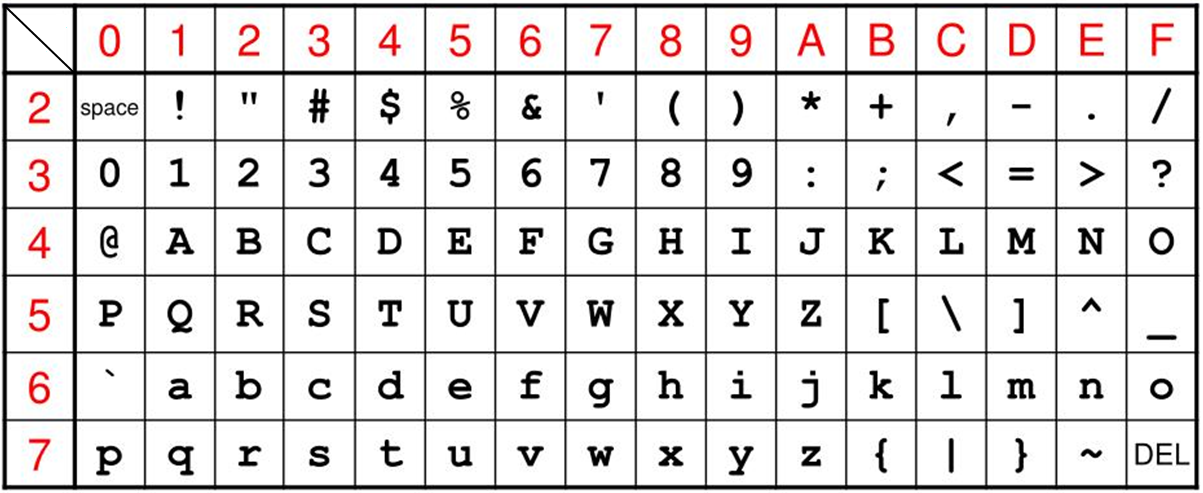
\includegraphics[width=\columnwidth]{ch-texte/img/ASCII.png}\\
    \textit{La table ASCII}
\end{center}
Le code ASCII se base sur un tableau contenant les caractères les plus utilisés en langue anglaise : les lettres de l'alphabet en majuscule (de A
à Z) et en minuscule (de a à z),
les dix chiffres arabes (de 0 à 9), des signes de ponctuation (point, virgule, point-virgule, deux points, points d'exclamation et
d'interrogation, apostrophe ou \textit{quote}, guillemet
ou \textit{double quotes}, parenthèses, crochets etc.), quelques symboles et certains caractères spéciaux invisibles (espace, retour-chariot,
tabulation, retour-arrière, etc.).\\

\begin{exercice}
    Combien y a -t-il de caractères dans ce catalogue ?\\
    Combien de bits sont nécessaires pour pouvoir représenter tous leurs numéros de code ?
\end{exercice}


Pour représenter ces symboles ASCII, les ordinateurs utilisaient des cases mémoires de un octet, mais ils réservaient toujours le huitième bit pour le contrôle de parité : c'est un procédé de sécurité pour
éviter les erreurs, qui étaient très fréquentes dans les premières mémoires électroniques.\\
\begin{methode}[ : contrôle d'erreur par parité]
    \begin{itemize}
        \item 	On dispose d'un mot de 7 bits, par exemple 111 0011
        \item 	On compte le nombre de bits à 1, il y en a 5.
        \item 	On rajoute le bit de poids fort à 1 pour qu'en tout, il y ait toujours \textit{un nombre pair} de bits à 1.\\
              On obtient \boxed{1}111 0011, ce bit de poids fort jouant le rôle de \textit{code correcteur}.
        \item 	Un autre exemple : 001 1110 est codé \boxed{0}001 1110.
    \end{itemize}
\end{methode}

\begin{exercice}[]
    Voici un message reçu à l'issue d'une transmission :
    \begin{center}
        \texttt{53 E1 6C F5 70}
    \end{center}
    Ces 6 octets sont censés représenter 6 caractères ASCII, codées sur 7 bits le 8\eme étant réservé au contrôle d'erreur par parité.
    \begin{enumerate}
        \item 	Décoder ces 6 octets en disant s'il y a des erreurs ou non.
        \item 	Quel était le message initial ?
    \end{enumerate}
\end{exercice}


\section{L'insuffisance de l'ASCII}

Pour coder les lettres accentuées, inutilisées en Anglais mais très fréquentes dans d'autres langues (notamment le Français), on a décidé
d'étendre
le codage des caractères au huitième bit (les erreurs-mémoire étant devenues plus rares et les méthodes de contrôle d'erreurs plus efficaces).\\


\begin{exercice}[]
    Combien de nouveaux symboles a-t-on pu coder en autorisant le huitième bit dans le codage ?
\end{exercice}


On a alors pu coder toutes ces lettres et ainsi que de nouveaux caractères typographiques utiles tels que différents tirets.\\


\section{Le problème}

Le fait d'utiliser un bit supplémentaire a bien entendu ouvert des possibilités mais malheureusement les caractères de toutes les langues ne
pouvaient être pris en charge
en même temps.\\
La norme ISO 8859–1 appelée aussi Latin-1 ou Europe occidentale est la première partie d'une norme plus complète appelée \textbf{ISO 8859} (qui
comprend 16 parties)
et qui permet de coder tous les caractères des langues européennes. Cette norme ISO 8859–1 permet de coder 191 caractères de l'alphabet latin qui
avaient à
l'époque été jugés essentiels dans l'écriture, mais omet quelques caractères fort utiles (ainsi, la ligature œ n'y figure pas).\\

Dans les pays occidentaux, cette norme est utilisée par de nombreux systèmes d'exploitation, dont Linux et Windows. Elle a donné lieu à quelques
extensions
et adaptations, dont \textbf{Windows-12527} (appelée \textbf{ANSI}) et ISO 8859-158 (qui prend en compte le symbole €\  créé après la norme
ISO 8859-1).
C'est une source de grande confusion pour les développeurs de programmes informatiques car un même caractère peut être codé différemment suivant
la norme utilisée .\\
Voici les tableaux décrivant deux encodages :

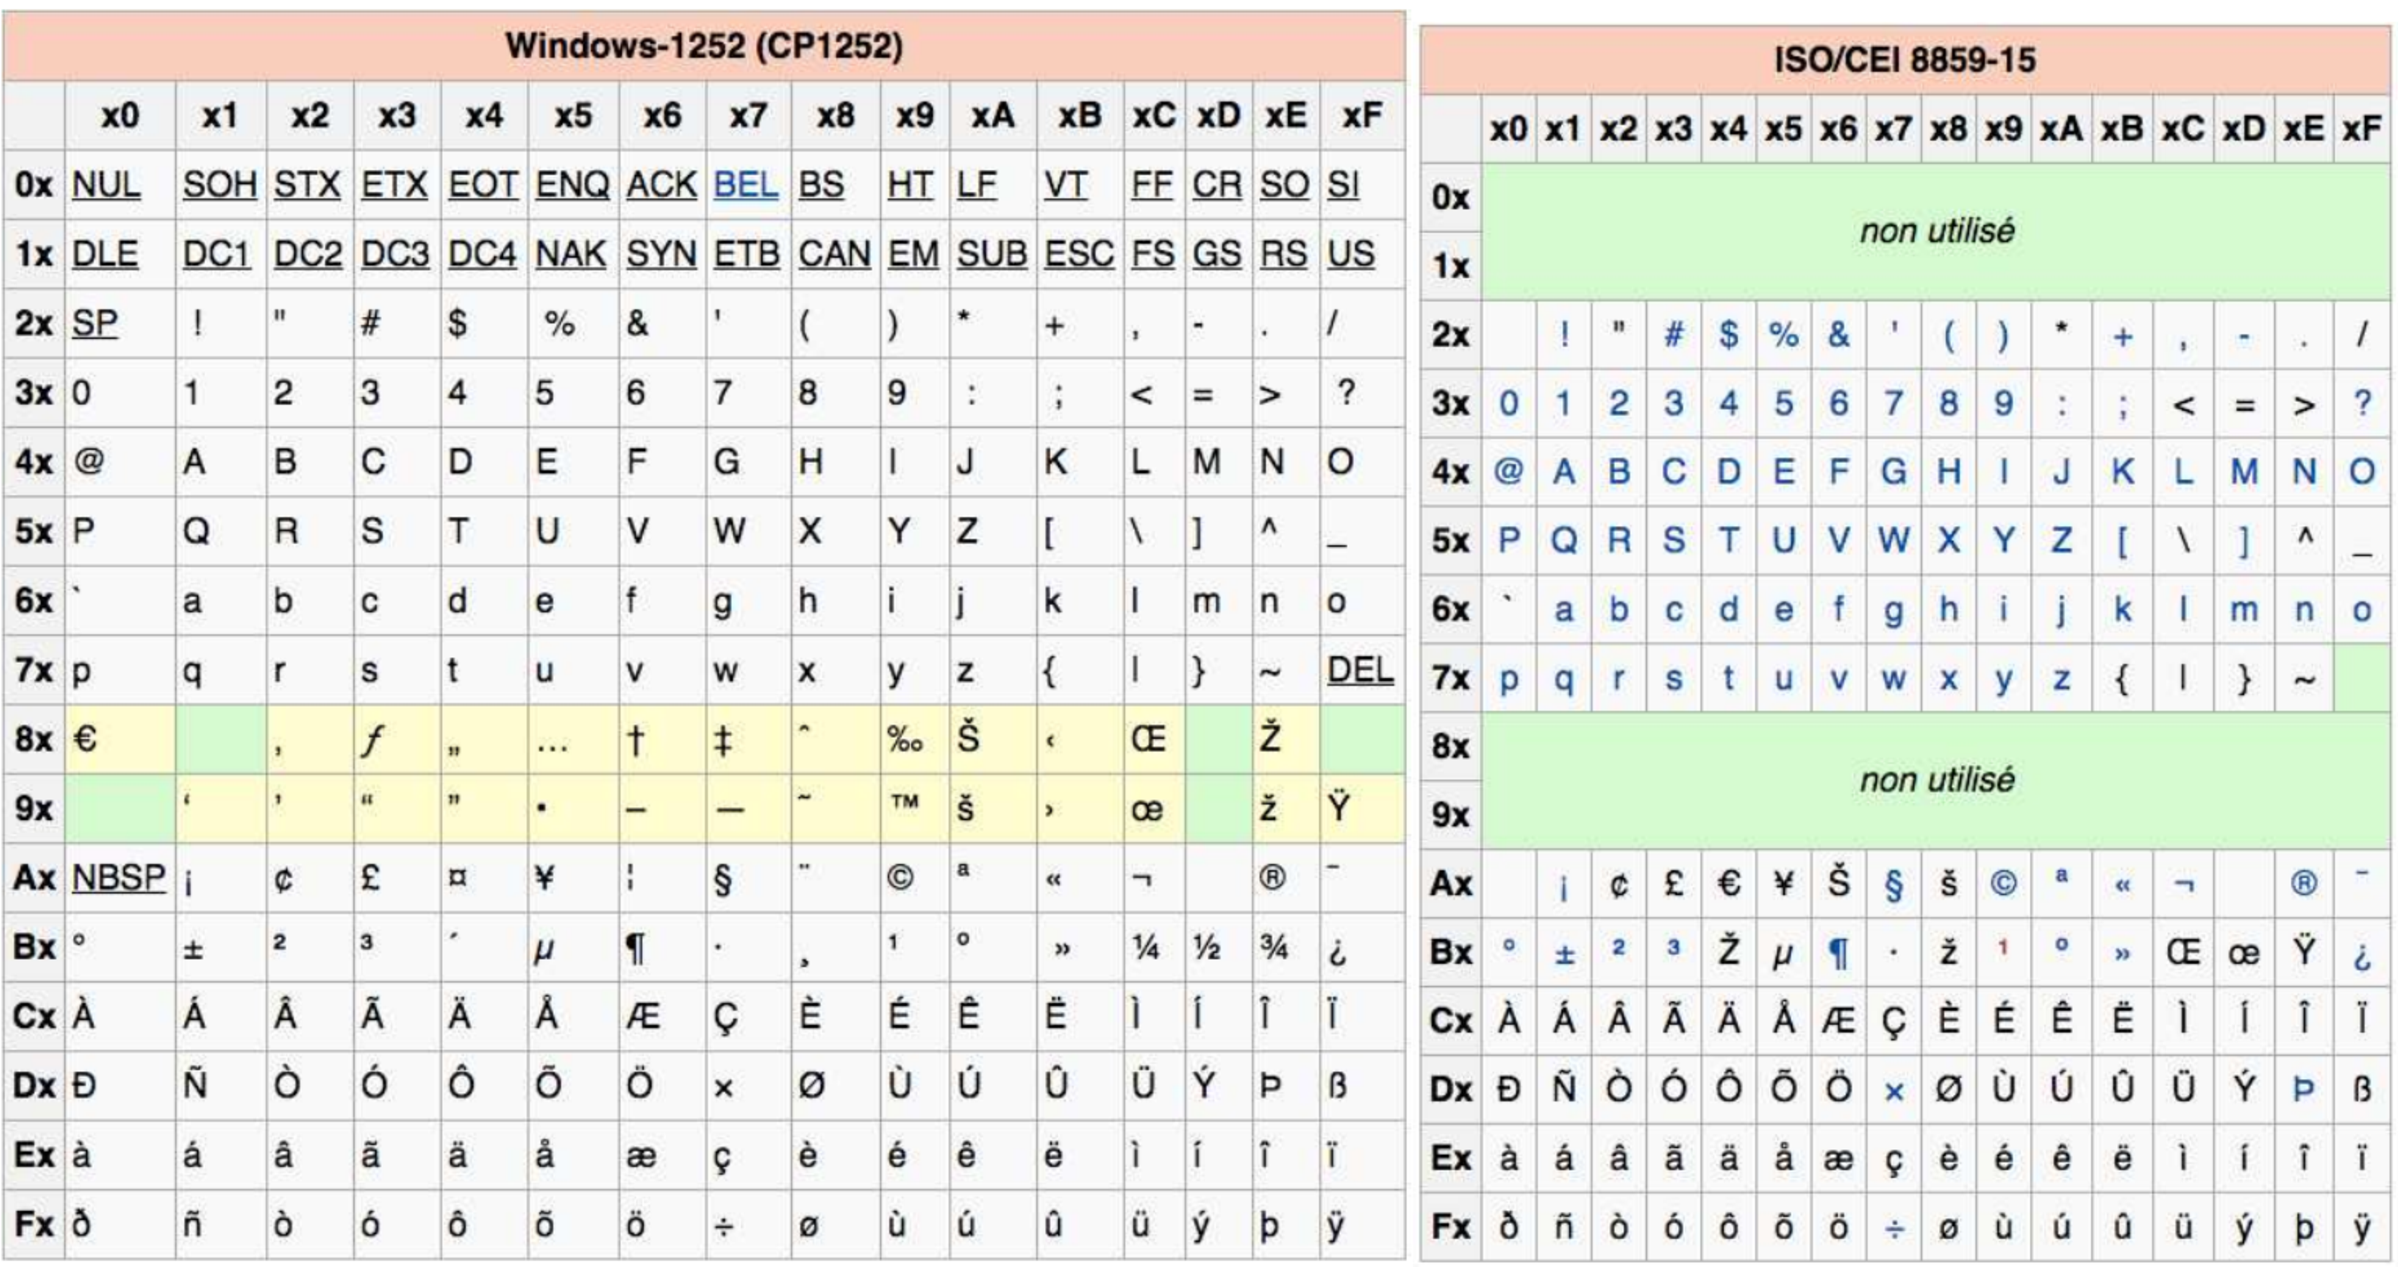
\includegraphics[width=\columnwidth]{ch-texte/img/W1252andISO}\\


\begin{exercice}[]
    Ces deux encodages sont-ils totalement compatibles ? Pourquoi ?
\end{exercice}

\section{La multiplicité des encodages}

Au fil du temps une multitude d'encodages sont apparus, multipliant les sources de confusion.\\
Voici pour l'exemple une partie des encodages que \textsc{Python} reconnaît :
\alternaterowcolors
\begin{center}
    {\tiny
        \begin{tabular}{CCC}
            
            \rowcolor{UGLiOrange}{\boxfont\color{white}Encodage} & {\boxfont\color{white}Alias Python}                                      & {\boxfont\color{white}Langues concernées}             \\
            
            ascii                                                & 646,us-ascii                                                             & English                                               \\
            big5                                                 & big5-tw, csbig5                                                          & Traditional Chinese                                   \\
            cp424                                                & EBCDIC-CP-HE, IBM424                                                     & Hebrew                                                \\
            cp437                                                & 437, IBM437                                                              & English                                               \\
            cp500                                                & EBCDIC-CP-BE, EBCDIC-CP-CH, IBM500                                       & Western Europe                                        \\
            cp720                                                &                                                                          & Arabic                                                \\
            cp737                                                &                                                                          & Greek                                                 \\
            cp856                                                &                                                                          & Hebrew                                                \\
            cp857                                                & 857, IBM857                                                              & Turkish                                               \\
            cp864                                                & IBM864                                                                   & Arabic                                                \\
            cp874                                                &                                                                          & Thai                                                  \\
            cp932                                                & 932, ms932, mskanji, ms-kanji                                            & Japanese                                              \\
            cp1251                                               & windows-1251                                                             & Bulgarian, Byelorussian, Macedonian, Russian, Serbian \\
            cp1258                                               & windows-1258                                                             & Vietnamese                                            \\
            euc\_kr                                              & euckr, korean, ksc5601, ks\_c-5601, ks\_c-5601-1987, ksx1001, ks\_x-1001 & Korean                                                \\
            gbk                                                  & 936, cp936, ms936                                                        & Unified Chinese                                       \\
            latin\_1                                             & iso-8859-1, iso8859-1, 8859, cp819, latin, latin1, L1                    & West Europe                                           \\
            iso8859\_14                                          & iso-8859-14, latin8, L8                                                  & Celtic languages                                      \\
            koi8\_r                                              &                                                                          & Russian                                               \\
            utf\_8                                               & U8, UTF, utf8                                                            & all languages                                         \\
        \end{tabular}}
\end{center}

\begin{exercice}[]
    Lequel de ces encodages semble le plus performant ?
\end{exercice}


\section{L'Unicode}

La globalisation des échanges culturels et économiques a mis l'accent sur le fait que les langues européennes coexistent avec de nombreuses
autres
langues aux alphabets spécifiques voire sans alphabet (le Japonais utilise entre autres un syllabaire, chaque symbole représentant une syllabe).
La
généralisation de l'utilisation d'Internet dans le monde a ainsi nécessité une prise en compte d'un
nombre beaucoup plus important de caractères (à titre d'exemple, le mandarin possède à lui tout seul plus de 5000 caractères !).\\
Une autre motivation pour cette
évolution résidait dans les possibles confusions dues au trop faible nombre de caractères pris en compte ; ainsi, les symboles monétaires des
différents
pays n'étaient pas tous représentés dans le système ISO 8859-1, de sorte que les ordres de paiement internationaux transmis par courrier
électronique
risquaient d'être mal compris. La norme Unicode a donc été créée pour permettre le codage de textes écrits quel que soit le système d'écriture
utilisé.\\

Dans le système UTF-8, on attribue à chaque caractère un nom, une position normative et un bref descriptif qui seront les mêmes quelle que soit
la plate-forme informatique
ou le logiciel utilisés.\\
Un consortium composé d'informaticiens, de chercheurs, de linguistes et de personnalités représentant les états ainsi que les entreprises
s'occupe d'unifier toutes les pratiques en un seul et même système : \textit{l'Unicode}.\\

\begin{definition}
    L'\textit{Unicode}  est  une table de correspondance Caractère-Code (Charset), et l'\textit{UTF-8} est l'encodage correspondant (Encoding) le
    plus répandu.
\end{definition}

De nos jours, par défaut, les navigateurs Internet utilisent le codage UTF-8 et les concepteurs de sites pensent de plus en plus à créer leurs
pages web
en prenant en compte cette même norme ; c'est pourquoi il y a de moins en moins de problèmes de compatibilité : l'UTF-8 est aujourd'hui
majoritairement utilisé pour les sites du web, comme le montre ce graphique.

\begin{center}
    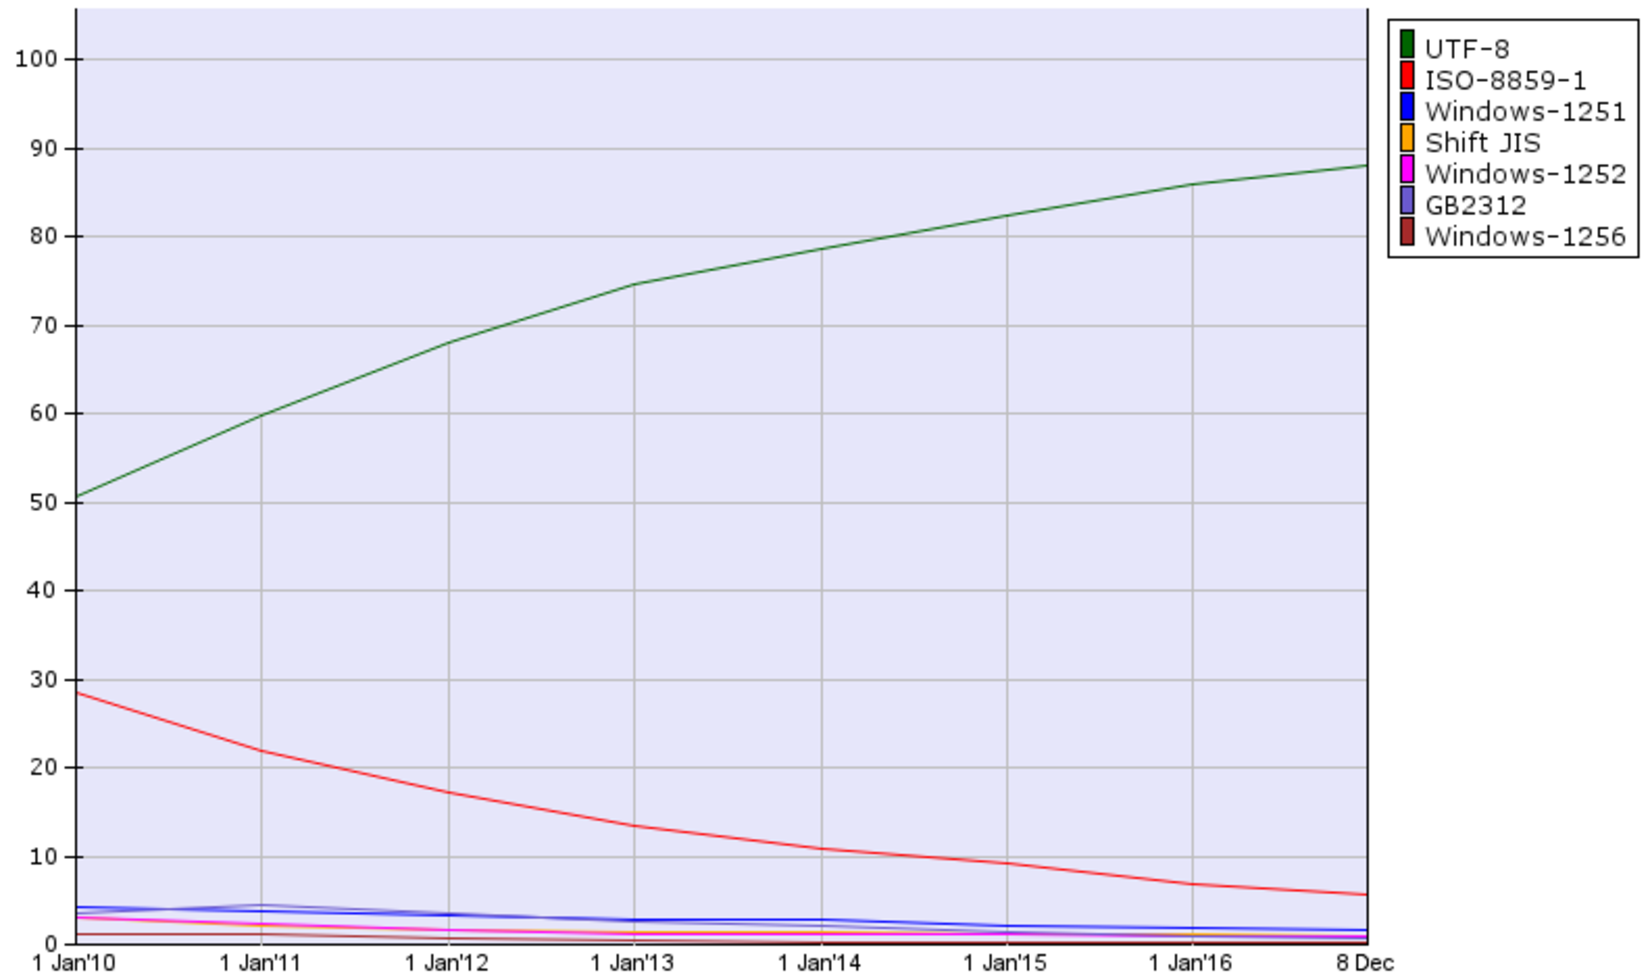
\includegraphics[width=10cm]{ch-texte/img/UTF8evol}
\end{center}

L'UTF-8 est également le codage le plus utilisé dans les systèmes GNU, Linux et compatibles pour gérer le plus simplement
possible des textes et leurs traductions dans tous les systèmes d'écritures et tous les alphabets du monde.\\

\section{L'UTF-8 côté technique}

La norme Unicode définit entre autres un ensemble (ou répertoire) de caractères. Chaque caractère est repéré dans cet ensemble par un index
entier aussi appelé « point de code ».\\
Par exemple le caractère « € » (euro) est le 8365$^{\text{ème}}$ caractère du répertoire Unicode, son index, ou point de code, est donc
8364
(on commence à compter à partir de 0).\\
Le répertoire Unicode peut contenir plus d'un million de caractères, ce qui est bien trop grand pour être codé par un seul octet (limité à des
valeurs entre 0 et 255).
La norme Unicode définit donc des méthodes standardisées pour coder et stocker cet index sous forme de séquence d'octets :
UTF-8 est la plus utilisée d'entre elles (il y a aussi des variantes comme UTF-16 et UTF-32).
En UTF-8, tout caractère est codé sur 1, 2, 3 ou 4 octets.\\
La principale caractéristique d'UTF-8 est qu'elle est \textit{rétro-compatible avec la norme ASCII}, c'est-à-dire que tout caractère ASCII se
code
en UTF-8 sous forme d'un unique octet, identique au code ASCII.\\
Par exemple « A » (A majuscule) a pour code ASCII 65 et se code en UTF-8 par l'octet 65, il en va de même pour tous les caractère ASCII.
Pour les autres, on procède comme ceci :
\begin{itemize}
    \item Chaque caractère est associé à son index Unicode.
    \item 	En général, cet index est exprimé en hexadécimal.
          Actuellement, presques toutes les valeurs de 0000 à FFFF, c'est-à-dire de 0 à 65535 sont
          attribuées à des \og alphabets \fg{} associés à des langues, des plus communes aux plus rares, et à divers symboles, tels que les
          symboles mathématiques.
          Au delà de FFFF on trouve des alphabets associés à des langues anciennes (cunéiformes, hiéroglyphes\ldots).
    \item  En fonction du nombre de bits nécessaires pour représenter en binaire  cet index, on utilise le codage suivant :\\

          \begin{center}
              {\scriptsize
                  \begin{tabular}{CCC}

                      \rowcolor{UGLiOrange}{\boxfont\color{white}Nombre de bits de l'index} & {\boxfont\color{white}Nombre d'octets pour coder en UTF-8} & {\boxfont\color{white}Schéma de codage}                                     \\

                      de 0 à 7                                                              & 1                                                          & 0xxx xxxx                                                                   \\

                      de 8 à 11                                                             & 2                                                          & \textbf{110}x xxxx \textbf{10}xx xxxx                                       \\

                      de 12 à 16                                                            & 3                                                          & \textbf{1110} xxxx \textbf{10}xx xxxx \textbf{10}xx xxxx                    \\

                      de 17 à 21                                                            & 4                                                          & \textbf{1111 0}xxx \textbf{10}xx xxxx \textbf{10}xx xxxx \textbf{10}xx xxxx \\
                  \end{tabular} }
              \normalsize
          \end{center}
          \vspace{1em}
\end{itemize}
Par exemple le symbole €\  a un index Unicode qui vaut 8364.\\
\begin{itemize}
    \item 	8364 s'écrit 20AC en hexa, ce qui fait 10 0000 1010 1100 en binaire, soit 14 bits.\\
          On va donc utiliser 3 octets pour coder, conformément au schéma de codage.
    \item 	On commence par écrire le mot de 16 bits correspondant : \boxed{00}10 0000 1010 1100.\\
    \item 	On formate comme à la 3ème ligne du tableau : \\

          \textbf{1110} 0010 \textbf{10}00 0010 \textbf{10}10 1100\\

          Ce qui fait 3 octets : E2 82 AC en hexadécimal.\\

\end{itemize}


\begin{exercice}[]
    Si un ordinateur lit cet encodage UTF-8 du symbole €\  selon l'encodage ISO8859-15, qu'affichera-t-il ?\\

\end{exercice}


\section{Conclusion}

Même si l'encodage UTF-8 devient le standard international, certains développeurs, sites, ou applications en utilisent malgré tout encore
d'autres.\\

\begin{propriete}
    La notion de texte brut n'existe pas en informatique : lorsqu'un ordinateur lit un fichier texte il n'a \textit{a priori} aucun moyen de savoir
    quel est son encodage.
\end{propriete}

Beaucoup de documents indiquent donc en en tête leur format d'encodage : en HTML, on écrira dans l'en-tête d'une page:
\begin{html}
    \begin{minted}{html}
        <meta charset="utf8"/>
    \end{minted}
\end{html}

pour préciser qu'elle est encodée en UTF-8.\\
\section{Et Python dans tout ça ?}
En \textsc{Python}, on pourra aussi écrire : \mintinline{python}{# -*- coding: utf8 -*-} en première ligne de tout script pour signifier la même chose, \textit{et c\ae tera}.\\

\textsc{Python} gère très bien les encodages. On peut fabriquer un convertisseur très rapidement :

\begin{pyc}
    \begin{minted}{python}
fichier = open("nom_fichier", 'rt', encoding="utf8")
texte = fichier.read()
fichier.close()
    \end{minted}
\end{pyc}

Ceci permet de lire le contenu d'un fichier texte (d'où le \mintinline{python}{'rt'}, pour 'read text') d'un fichier texte encodé en UTF-8, et de le stocker dans la
variable \texttt{texte}, de type \mintinline{python}{str}.\\

\begin{pyc}
    \begin{minted}{python}
fichier = open("nom_fichier", 'wt', encoding="utf8")
fichier.write("Salut")
fichier.close()	
    \end{minted}
\end{pyc}

Permet d'écrire un fichier texte (d'où le \mintinline{python}{'wt'}, pour write text) en UTF-8.\\

\section{Exercices}
\begin{exercice}
    Analyser les deux fichiers \texttt{texte1(utf8).txt} et \texttt{texte1(utf8).txt} : ils sont tous les deux encodés en UTF-8.


    \begin{itemize}
        \item Ouvrir chaque fichier. Quelles sont les différences de contenu entre ces deux fichiers ?
        \item Faire un clic droit puis \texttt{Propriétés} comme ceci :\\

              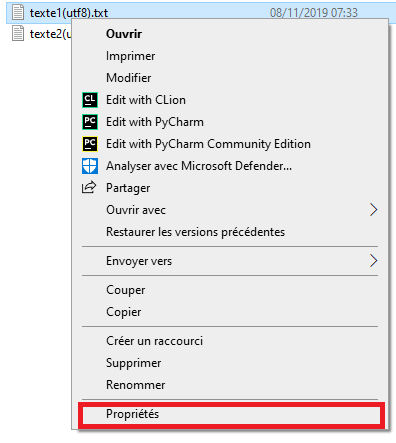
\includegraphics[width=7cm]{ch-texte/img/expli1}\\

              Quelles sont les tailles de ces deux fichiers ?\\
              Comment, dans le détail, la différence de taille s'explique-t-elle ?

    \end{itemize}
\end{exercice}

\begin{exercice} Nous allons examiner des problèmes d'encodage.
    \begin{itemize}
        \item Ouvrir le fichier \texttt{index1(utf8).html} avec un navigateur, puis le fichier \texttt{index2(utf8).html} avec un navigateur.\\
              Que remarquez-vous ?\\

        \item 	Ouvrir ce dernier fichier avec un éditeur de texte (comme le bloc-notes Windows).\\
              D'où vient le problème ? Proposer une correction.\\
              Expliquer en détail pourquoi à la place des \og é \fg{}, il y a des \og é \fg{} .\\

        \item 	Ouvrir le fichier \texttt{index3(ISO8859-15).html} avec un navigateur.\\
              D'où vient le problème ? Proposer une correction.\\
              Expliquer en détail pourquoi il y a des \og points d'interrogation dans des losanges noirs \fg{}.\\
    \end{itemize}
\end{exercice}

\begin{exercice}
    \'Ecrire un script qui corrige le problème de  \texttt{index3(ISO8859-15).html} en le convertissant en UTF-8 (utiliser les scripts \textsc{Python} fournis à la section précédente).

\end{exercice}